\section{Experiment 1: Diode Characteristics}

\subsection{Objective}
The objective of this experiment is to study the characteristics of a semiconductor diode, including its I-V relationship, and to demonstrate its applications in rectification circuits.

\subsection{Theory}
A diode is a two-terminal electronic component that conducts current primarily in one direction. It is made of semiconductor material with a p-n junction. The current-voltage (I-V) characteristic of a diode is described by the Shockley diode equation:

\[
I = I_s \left( e^{\frac{V_d}{n V_t}} - 1 \right)
\]

where:
- \(I\) is the diode current,
- \(I_s\) is the reverse saturation current,
- \(V_d\) is the voltage across the diode,
- \(n\) is the ideality factor (typically 1-2),
- \(V_t = \frac{kT}{q}\) is the thermal voltage (approximately 26 mV at room temperature).

For small forward voltages, the diode behaves exponentially, while in reverse bias, the current is approximately \(-I_s\).

\subsubsection{Applications}
Diodes have several applications in electronic circuits:
- \textbf{Rectification}: Converting AC to DC using half-wave or full-wave rectifiers.
- \textbf{Clipping and Clamping}: Shaping waveforms by removing parts of the signal.
- \textbf{Voltage Regulation}: Using Zener diodes to maintain constant voltage.
- \textbf{Switching}: In digital circuits for logic operations.
- \textbf{Signal Modulation}: In AM demodulators.

\subsubsection{Waveforms}
In a half-wave rectifier, the input is a sinusoidal AC voltage, and the output is the positive half-cycles, resulting in a pulsating DC with ripple.

\begin{figure}[H]
    \centering
    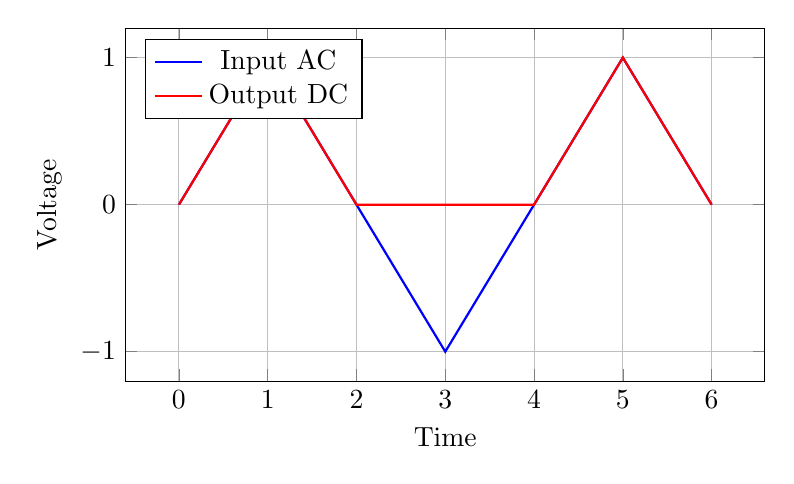
\begin{tikzpicture}
        \begin{axis}[
            width=0.8\textwidth,
            height=0.5\textwidth,
            xlabel={Time},
            ylabel={Voltage},
            grid=major,
            legend pos=north west
        ]
        \addplot[blue, thick] coordinates {(0,0) (1,1) (2,0) (3,-1) (4,0) (5,1) (6,0)};
        \addlegendentry{Input AC}
        \addplot[red, thick] coordinates {(0,0) (1,1) (2,0) (3,0) (4,0) (5,1) (6,0)};
        \addlegendentry{Output DC}
        \end{axis}
    \end{tikzpicture}
    \caption{Half-wave rectifier waveforms.}
    \label{fig:waveforms}
\end{figure}

\subsubsection{Reference}
Sedra, A. S., \& Smith, K. C. (2016). Microelectronic Circuits (7th ed.). Oxford University Press.

\subsection{Apparatus}
- Semiconductor diode (e.g., 1N4001)
- DC power supply
- Multimeter (for voltage and current measurement)
- Resistors (various values)
- Connecting wires
- Breadboard

\subsection{Schematic Diagrams}
\subsubsection{I-V Characteristic Circuit}
\begin{figure}[H]
    \centering
    \begin{circuitikz}
        \draw (0,0) to [V, v=$V_s$] (0,2);
        \draw (0,2) to [R, l=$R_1$] (2,2);
        \draw (2,2) to [diode, l=$D_1$] (2,0);
        \draw (2,0) to (0,0);
        \draw (2,2) to [ammeter] (4,2);
        \draw (2,0) to [voltmeter] (4,0);
    \end{circuitikz}
    \caption{Circuit for measuring diode I-V characteristics.}
    \label{fig:iv_circuit}
\end{figure}

\subsubsection{Half-Wave Rectifier Circuit}
\begin{figure}[H]
    \centering
    \begin{circuitikz}
        \draw (0,0) to [sinusoidal voltage source, v=$V_{in}$] (0,2);
        \draw (0,2) to [diode, l=$D_1$] (2,2);
        \draw (2,2) to [R, l=$R_L$] (2,0);
        \draw (2,0) to (0,0);
    \end{circuitikz}
    \caption{Half-wave rectifier circuit.}
    \label{fig:rectifier}
\end{figure}

\subsection{Scaled Graphs}
The I-V characteristic of the diode is plotted below.

\begin{figure}[H]
    \centering
    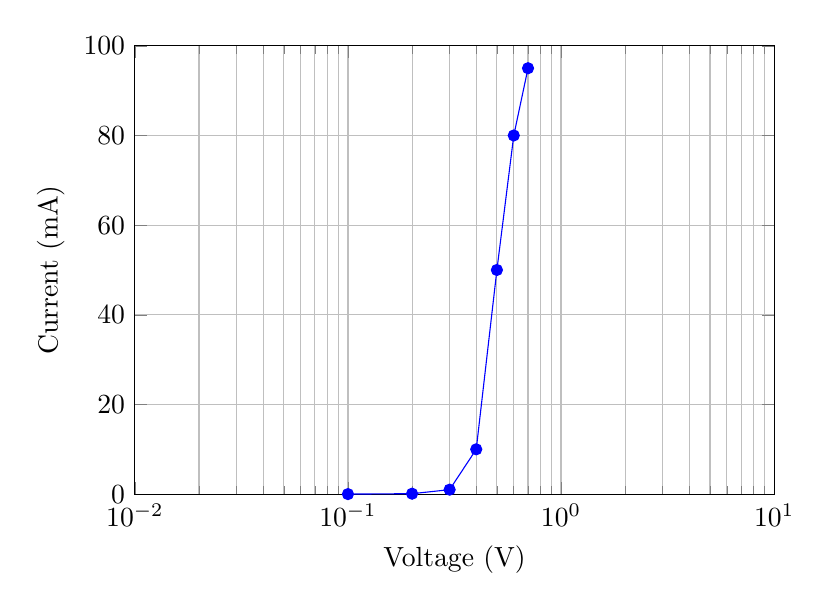
\begin{tikzpicture}
        \begin{semilogxaxis}[
            width=0.8\textwidth,
            height=0.6\textwidth,
            xlabel={Voltage (V)},
            ylabel={Current (mA)},
            grid=both,
            xmin=0.01, xmax=10,
            ymin=0, ymax=100
        ]
        \addplot[blue, mark=*] coordinates {
            (0.1, 0.01)
            (0.2, 0.1)
            (0.3, 1)
            (0.4, 10)
            (0.5, 50)
            (0.6, 80)
            (0.7, 95)
        };
        \end{semilogxaxis}
    \end{tikzpicture}
    \caption{Diode I-V characteristic (sample data).}
    \label{fig:iv_plot}
\end{figure}

\subsection{Observations}
The following table shows the measured voltage and current values for the diode.

\begin{table}[H]
    \centering
    \caption{Diode I-V Measurements}
    \begin{tabular}{|c|c|}
        \hline
        Voltage (V) & Current (mA) \\
        \hline
        0.1 & 0.01 \\
        \hline
        0.2 & 0.1 \\
        \hline
        0.3 & 1 \\
        \hline
        0.4 & 10 \\
        \hline
        0.5 & 50 \\
        \hline
        0.6 & 80 \\
        \hline
        0.7 & 95 \\
        \hline
    \end{tabular}
    \label{tab:observations}
\end{table}

\subsection{Explanation of Results}
The I-V characteristic plot shows the exponential increase in current with forward voltage, starting from a small reverse saturation current at negative voltages. This behavior aligns with the Shockley diode equation, where the current rises sharply once the voltage exceeds the threshold (around 0.7 V for silicon diodes). The semilogarithmic scale highlights the exponential nature, with the curve bending upwards as voltage increases.

For the half-wave rectifier, the waveform demonstrates how the diode allows only positive half-cycles to pass, blocking the negative ones. This results in a pulsating DC output with ripple, which can be smoothed using capacitors in practical applications. The observed output matches theoretical expectations, confirming the diode's role in rectification.

\subsection{Conclusion}
The experiment successfully demonstrated the exponential I-V characteristic of the diode, confirming the Shockley equation. The rectifier circuit produced the expected half-wave output, validating the diode's rectification application. The objectives were met, providing insight into diode behavior for practical electronic designs.